\documentclass[12pt,a4paper]{amsart}
% ukazi za delo s slovenscino -- izberi kodiranje, ki ti ustreza
\usepackage[slovene]{babel}
%\usepackage[cp1250]{inputenc}
\usepackage[T1]{fontenc}
\usepackage[utf8]{inputenc}
\usepackage{amsmath,amssymb,amsfonts}
\usepackage{url}
%\usepackage[normalem]{ulem}
\usepackage[dvipsnames,usenames]{color}
\usepackage{pgf}
\usepackage{tikz}
\usepackage{graphicx}
\usepackage{bbm}
\usepackage{hyperref}
\hypersetup{
    colorlinks=true, %set true if you want colored links
    linktoc=all,     %set to all if you want both sections and subsections linked
    linkcolor=black,  %choose some color if you want links to stand out
}

\tikzstyle{block} = [rectangle, draw, 
    text width=8em, text centered, rounded corners, minimum height=4em]
\tikzstyle{line} = [draw, -latex]

% ne spreminjaj podatkov, ki vplivajo na obliko strani
\textwidth 15cm
\textheight 24cm
\oddsidemargin.5cm
\evensidemargin.5cm
\topmargin-5mm
\addtolength{\footskip}{10pt}
\pagestyle{plain}
\overfullrule=15pt % oznaci predlogo vrstico


% ukazi za matematicna okolja
\theoremstyle{definition} % tekst napisan pokoncno
\newtheorem{definicija}{Definicija}[section]
\newtheorem{primer}[definicija]{Primer}
\newtheorem{opomba}[definicija]{Opomba}

\renewcommand\endprimer{\hfill$\diamondsuit$}


\theoremstyle{plain} % tekst napisan posevno
\newtheorem{lema}[definicija]{Lema}
\newtheorem{izrek}[definicija]{Izrek}
\newtheorem{trditev}[definicija]{Trditev}
\newtheorem{posledica}[definicija]{Posledica}
\newtheorem{zgled}[definicija]{Zgled}
\newtheorem{hipoteza}[definicija]{Hipoteza}


% za stevilske mnozice uporabi naslednje simbole
\newcommand{\R}{\mathbb R}
\newcommand{\N}{\mathbb N}
\newcommand{\Z}{\mathbb Z}
\newcommand{\C}{\mathbb C}
\newcommand{\Q}{\mathbb Q}

% ukaz za slovarsko geslo
\newlength{\odstavek}
\setlength{\odstavek}{\parindent}
\newcommand{\geslo}[2]{\noindent\textbf{#1}\hspace*{3mm}\hangindent=\parindent\hangafter=1 #2}

% naslednje ukaze ustrezno popravi
\newcommand{\program}{Finančna matematika} % ime studijskega programa: Matematika/Finan"cna matematika
\newcommand{\imeavtorja}{Tim Kalan} % ime avtorja
\newcommand{\imementorja}{izr.~prof.~dr. Marjetka Knez} % akademski naziv in ime mentorja
\newcommand{\naslovdela}{Spodbujevalno učenje pri igranju namiznih iger}
\newcommand{\letnica}{2021} %letnica diplome


% vstavi svoje definicije ...




\begin{document}

% od tod do povzetka ne spreminjaj nicesar
\thispagestyle{empty}
\noindent{\large
UNIVERZA V LJUBLJANI\\[1mm]
FAKULTETA ZA MATEMATIKO IN FIZIKO\\[5mm]
\program\ -- 1.~stopnja}
\vfill

\begin{center}{\large
\imeavtorja\\[2mm]
{\bf \naslovdela}\\[10mm]
Delo diplomskega seminarja\\[1cm]
Mentorica: \imementorja}
\end{center}
\vfill

\noindent{\large
Ljubljana, \letnica}
\pagebreak

\thispagestyle{empty}
\tableofcontents
\pagebreak

\thispagestyle{empty}
\begin{center}
{\bf \naslovdela}\\[3mm]
{\sc Povzetek}
\end{center}
% tekst povzetka v slovenscini
V povzetku na kratko opišite vsebinske rezultate dela. Sem ne sodi razlaga organizacije
dela -- v katerem poglavju/razdelku je kaj, pa"c pa le opis vsebine.
\vfill
\begin{center}
{\bf Reinforcement learning in board games}\\[3mm] % prevod slovenskega naslova dela 
{\sc Abstract}
\end{center}
% tekst povzetka v anglescini
Prevod zgornjega povzetka v angle"s"cino.

\vfill\noindent
{\bf Math. Subj. Class. (2010):} navedite vsaj eno klasifikacijsko oznako -- 
        dostopne so na \url{www.ams.org/mathscinet/msc/msc2010.html}  \\[1mm]  
{\bf Ključne besede:} Spodbujevalno učenje, Markovski proces odločanja  \\[1mm]  
{\bf Keywords:} Reinforcement learning, Markov decision process
\pagebreak



% tu se zacne tekst seminarja
\section{Uvod}
%Na za"cetku prvega poglavja/razdelka (ali v samostojnem razdelku z naslovom Uvod) napi"site 
%kratek zgodovinski in matemati"cni uvod. Pojasnite motivacijo za problem, kje nastopa, kje 
%vse je bil obravnavan. Na koncu opi"site tudi organizacijo dela -- kaj je v kak"snem razdelku.
%
%"Ce se uvod naravno nadaljuje v besedilo prvega poglavja, lahko nadaljujete z besedilom v istem 
%razdelku, sicer za"cnete novega. Na za"cetku vsakega razdelka/podraz\-delka povete, "cemu se 
%bomo posvetili v nadaljevanju. Pri pisanju uporabljajte ukaze za matemati"cna okolja, med 
%formalnimi enotami dodajte vezni razlagalni tekst.
Namizne igre ljudje igramo že od prazgodovine. Na Kitajskem je bila igra Go znana kot ena 
izmed štirih umetnosti Kitajskega učenjaka poleg igranja inštrumenta s strunami, kaligrafije
in slikanja. Spremljajo nas že zelo dolgo časa, zato je naravno, da jih želimo ljudje čim
bolje igrati.

Z adventom računalnika in računalništva je bil ta problem postavljen v novi luči. Vprašanje
ni bilo več samo, kako dobro lahko človek igra igro sam, temveč tudi do kakšnega nivoja 
lahko spravi računalnik. Izkazalo se je, da nam pri tem problemu (in mnogih drugih) zelo dobro
koristi ">umetna inteligenca"< oz. metode strojnega učenja (SU). Eno izmed vej SU bomo 
predstavili v tem delu in pogledali, kako nam lahko pomaga pri igranju namiznih iger.

Ideja, da bi nek stroj igral igre, ni nova, in kompleksnosti takega stroja so se zavedali ljudje
že pred obstojem računalnika. 
Za konec uvodnega dela morda zabeležimo še citat iz eseja ameriškega pisatelja in pesnika 
Edgarja Allana Poea, ki govori o mehaničnem igralcu šaha: 

\begin{quotation}
    %“If we choose to call the former 
    %[Chess-Player] a pure machine we must be prepared to admit that it is, beyond all comparison, 
    %the most wonderful of the inventions of mankind.”
    ">Če prej omenjenemu [igralcu šaha] rečemo čisti stroj, moramo biti pripravljeni priznati, da je
    zunaj vseh primerjav, najbolj čudovit izum človeštva."<
\end{quotation}

\subsection{Motivacija}
Spodbujevalno učenje ima zelo lepo motivacijo, in sicer izhaja iz psihologije. Znana psihologa 
Thorndike in Skinner, sta na živalih izvajala eksperimente; postavila sta jih v neko novo 
situacijo, kjer je lahko žival naredila akcijo, ki je rezultirala v neki nagradi. Ko je bila
žival ponovno postavljena v to situacijo, je hitreje ugotovila, katero akcijo mora storiti, da
pride do nagrade.

Koncept, ki je opisan v zgornjem odstavku, se imenuje instrumentalno pogojevanje. Z njim se 
srečamo tudi ljudje; tako se namreč učijo otroci, odrasli ljudje pa se bolj zanesejo na 
logično razmišljanje. Vseeno pa je to motiviralo utemeljitelje spodbujevanega učenja

\subsection{Strojno učenje}
To relativno novo raziskovalno področje se deli na tri glavne veje:
\begin{itemize}
    \item \textbf{Nadzorovano učenje} se ukvarja s tem, kako iz nekih označenih podatkov 
            naučimo računalnik, da prepoznava razne signale (slike, govor, tekst, ...)
            in to znanje uporabi za razpoznavo novih, neoznačenih podatkov.
    \item \textbf{Nenadzorovano učenje} odstrani označevanje iz podatkov in v njih poskuša 
            odkriti skrite vzorce.
    \item \textbf{Spodbujevalno učenje} se ukvarja z ">učenjem iz izkušenj"<.
\end{itemize}

\subsection{Struktura naloge}
% morda to malo oštevilči
Naloga je razdeljena na štiri glavne dele. Na začetku so predstavljeni osnovni koncepti 
spodbujevalnega učenja in nekateri glavni algoritmi s tega področja. Potem se osredotočimo na 
na namizne igre in ob nekaj malega teorije iger povzamemo osnovne koncepte, na katere naletimo. 
V naslednjem odseku združimo znanje iz prejšnjih dveh in predstavimo, kako nam teorija iger 
pripomore pri spodbujevalnem učenju v tem konteksu. Na koncu pa so predstavljeni nekateri empirični
rezultati, ki sledijo iz zgoraj navedene teorije.

\section{Spodbujevalno učenje}
Spodbujevalno učenje se ukvarja s t. i. učenjem iz interakcije oz. izkušenj. Čeprav se to na prvi 
pogled ne zdi kot računska metoda, pač pa stvar psihologije, bomo kmalu dognali, kako prevesti 
to idejo v računalniku razumljiv jezik.

\subsection{Osnovni koncepti}
V osnovi nas zanima precej preprosta stvar: kako preslikati neko opazovano situacijo v akcijo na 
tak način, da učenec, ki mu v spodbujevalnem učenju pravimo \textbf{agent}, maksimizira neko 
numerično nagrado. Pri tem ne obstaja opazovalec, ki bi agentu povedal ali pa namignil, katere 
akcije so dobre, to mora ugotoviti sam, s poskušanjem in napakami. V tem dejstvu se skriva 
bistvena razlika med spodbujevalnim učenjem in ostalimi vejami strojnega učenja. 

Pomembna razlika tiči tudi v pomembnosti časa pri spodbujevalnem učenju. Pri drugih oblikah 
strojnega učenja se ponavadi ukvarjamo s tabelaričnimi podatki, tu pa ponavadi modeliramo nek 
dinamičen proces, zato je naravno, da je pomemben čas. Čeprav se ga da v tem kontekstu 
modelirati zvezno, je za naše namene dovolj, da ga opazujemo kot diskretne točke $t \in 
\{1, \dots, T\} $, kjer $T$ označuje nek končni čas (v splošnem je lahko seveda $T = \infty$).

\subsubsection{Nagrada}
Prvi pomemben koncept pri spodbujevanem učenju je nagrada. Kot smo že zgoraj omenili, to za nas 
pomeni neko numerično vrednost, kjer pozitivno število indicira ">pozitivno nagrado"<, negativno pa 
">kazen"<. S pomočjo tega koncepta formaliziramo \textit{cilj} učenja. Edini cilj agenta je 
maksimizacija te nagrade, pri čemer je vredno omeniti, da na nagrado agent lahko vpliva samo 
s svojimi akcijami (ne more recimo spremeniti načina, na katerega dobi nagrado). 

Posebej pomembno je na tem mestu poudariti, da akcije nimajo nujno neposredne nagrade. Le-te 
lahko pridejo v poljubnem kasnejšem časovnem obdobju. To je smiselno, če gledamo z vidika 
namiznih iger: pri šahu ne razmišljamo samo o neposrednih akcijah, temveč razvijamo neko 
dolgoročno strategijo, ki nas na koncu nagradi z zmago. 

\begin{zgled}[Križci in krožci]
    Pri tej znani otroški igri (in pri mnogo drugih namiznih igrah) modeliramo nagrado na 
    preprost način: če zmagamo, prejmemo nagrado $1$, če izgubimo pa $-1$. V vseh ostalih 
    situacijah, torej za izenačenje in po vsaki potezi, prejmemo nagrado $0$.
\end{zgled}

Zavedati se moramo tudi potencialnih omejitev oz. pomanjkljivosti takega modela. 
\begin{hipoteza}[Hipoteza o nagradi]
    Vse cilje je mogoče opisati kot maksimizacijo neke kumulativne numerične 
    nagrade.
\end{hipoteza}

\begin{zgled}[Protiprimera hipotezi o nagradi]
    Problem je, da hipoteza dovoljuje samo enodimezionalnost:
    \begin{itemize}
        \item Ko kupujemo hamburger, nam je pomemben okus in cena; kaj nam več pomeni?
        \item Država želi med epidemijo ohraniti življenja in gospodarstvo; v kakšni 
                meri naj prioritizira ti dve katergoriji?
    \end{itemize}
    Na tem mestu poudarimo še, da se da tudi v takih situacijah modelirati nagrado na zgoraj 
    opisani način in da je ta koncept vseeno dovolj splošen, da zajame zelo velik razred problemov.
    
\end{zgled}

\subsubsection{Okolje}
Okolje predstavlja del našega sistema, na katerega agent nima nobenega vpliva. Funkcija okolja
je, da agentu pokaže \textbf{stanje} (angl. \textit{state}) in mu da nagrado glede na 
\textbf{akcijo}, ki jo prejme od njega. Če se ponovno osredotočimo na namizne igre, bi lahko rekli, 
da je okolje igralna plošča \textit{in} nasprotnik  - tudi nanj namreč nimamo vpliva. Okolje nam 
služi tudi kot sodnik akcij oz. stanj. V kontekstu programa za igranje iger torej okolje izbira 
nasprotnikove akcije, odloča katero stanje pomeni zmago in dodeljuje nagrade.

\begin{zgled}[Križci in krožci]
    Okolje za nas pomeni $3\times3$ igralno polje \textbf{in} našega nasprotnika.
\end{zgled}

\subsubsection{Agent}
Kot smo že omenili zgoraj, je agent naš učenec. Njegov cilj je torej maksimizacija numerične 
nagrade, to težnjo pa dosega s pomočjo \textbf{strategije} (angl. \textit{policy}), ki mu pove, 
katero akcijo naj izbere v določenem stanju. Za ocenjevanje stanja si pomaga z \textbf{vrednostno 
funkcijo} (angl. \textit{value function}). Kot ime implicira, je to funkcija, ki določa vrednosti 
stanjem (in akcijam). 

Nagrada nam pove takojšnjo vrednost stanja, vrednostna funkcija pa to vrednost gleda na dolgi
rok. Je izpeljanka nagrade, a veliko bolj primerna za maksimizacijo kot nagrada, saj upošteva,
da so tudi stanja, ki ne prinesejo takojšnje nagrade, lahko veliko vredna.

Poleg tega je v splošnem lažje učenje prek vrednostnih funkcij kot prek strategij neposredno, 
saj je ponavadi stanj mnogokrat manj kot možnih strategij agenta.

Zapišimo zgoraj opisane pojme bolj formalno:

\begin{definicija}
    Naj $\mathcal{S}$ označuje množico vseh stanj, $\mathcal{A}$ pa množico vseh akcij. Naj $R_t,
    S_t, A_t$ zaporedoma označujejo nagrado, stanje in akcijo ob času $t$. Definiramo naslednje 
    pojme: 
    \begin{itemize}
        \item   Agentova \textbf{strategija} (angl. \textit{policy}) je v osnovi preslikava, ki 
                agentu pove, katero akcijo naj izbere v katerem stanju. Strategije delimo v dve 
                skupini:
                \begin{itemize}
                    \item \textbf{Deterministična strategija} je preslikava $\pi: \mathcal{S} 
                    \rightarrow \mathcal{A}$, ki za vsako stanje pove, katero akcijo agent v njem 
                    izbere
                    $$
                    a = \pi(s).
                    $$
                    \item \textbf{Stohastična strategija} je preslikava $\pi: \mathcal{A} \times 
                    \mathcal{S} \rightarrow [0, 1]$ ki za vsako stanje pove verjetnost, da se igra 
                    določena akcija. To označimo 
                    $$
                    \pi(a | s) = P(A_t = a~|~S_t = s).
                    $$
                \end{itemize}
                Seveda lahko vsako deterministično strategijo predstavimo kot stohastično, kjer je 
                verjetnost akcije $a$ $1$, verjetnosti ostalih akcij pa so enake $0$.
        
        \item Naj bodo $R_{t+1}, ...,R_T$ nagrade, ji jih bomo prejeli od trenutka 
                $t$ do končnega časa $T$. \textbf{Povračilo} (angl. \textit{return}) $G_t$ v splošnem
                definiramo za $T=\infty$,
                $$
                G_t = R_{t+1} + \gamma R_{t+2} + ... = \sum_{k=0}^\infty \gamma^k R_{t + k + 1} ,
                $$
                kjer je $\gamma \in [0,1]$ \textit{diskontni faktor}. Predstavlja dejstvo, da 
                imamo raje nagrade, ki bodo prišle prej. Formalno gledano, je cilj učenja 
                maksimizacija pričakovanega povračila.

         \item Naj bo $\pi$ dana strategija agenta. \textbf{Vrednostna funkcija 
                stanja} (angl. \textit{state value function}) glede na strategijo $\pi$ je
                $$
                v_\pi(s) = \mathrm{E} [G_t~|~S_t = s].
                $$
                Predstavlja torej pričakovani izplen, če se vedemo skladno s strategijo $\pi$.

        \item Naj bo $\pi$ še vedno dana strategija agenta. \textbf{Vrednostna funkcija 
                akcije} (tudi stanja-akcije) (angl. \textit{action value function}) glede na 
                strategijo $\pi$ je definirana kot
                $$
                q_\pi(s, a) = \mathrm{E} [G_t~|~S_t = s, A_t = a].
                $$
                Pove nam pričakovani izplen, če ob času $t$ naredimo akcijo $a$, nato pa se 
                vedemo skladno s strategijo $\pi$.
    \end{itemize}
\end{definicija}

\begin{zgled}[Križci in krožci]
    Agent je v tem primeru računalniški program, ki prejme igralno ploščo, nasprotnikove 
    poteze in nagrade, vrne pa optimalno strategijo (to si želimo).
\end{zgled}

\subsubsection{Model}
Model je nenujen del našega sistema. Predstavlja znanje, ki ga ima agent o svojem okolju. 
Če imamo model, da lahko uporabimo, ga napovemo, kako se bo vedlo okolje in s tem premaknemo
agentovo učenje iz čistih poskusov in napak na \textit{načrtovanje} (angl. \textit{planning}).
Model je torej poleg strategije in vrednostne funkcije še tretja komponenta agenta. Na podlagi 
modela lahko agent ">preračuna"< smiselnost svojih akcij, brez da bi dejansko karkoli storil. 

Prisotnost modela je glavna ločnica med dvema velikima, a zelo različnima vejama spodbujevalnega
učenja. Če modela ni, govorimo o spodbujevalnem učenju brez modela (angl. \textit{model-free 
reinforcement learning}), v nasprotnem primeru pa govorimo o učenju z modelom (angl. \textit
{model-based reinfocement learning}).

\subsection{Korak spodbujevalnega učenja}
Spodbujevalno učenje se pogosto ukvarja s procesi, ki naravno razpadejo v t. i. \textbf{epizode}. 
Tak proces so recimo namizne igre, kjer so epizode precej naravno posamezne igre. Ni pa nujno, 
da je delitev tako naravna (ali pa sploh možna oz. smiselna). Za namene te diplomske naloge lahko 
privzamemo, da taka delitev obstaja.

Ideja učenja je, da agenta spustimo v okolje in mu dovolimo, da doživi (igra) mnogo epizod. Nato 
na nek način (bo razjasnjeno kasneje) ob nekih določenih časih (npr. po koncu epizode) posodobi 
svojo strategijo (in/ali vrednostno funkcijo). 

Dejanski korak (npr. poteza v namizni igri) v epizodi pa formalno gledano opredelimo na naslednji 
način.
\begin{itemize}
    \item Agent naredi akcijo $A_t$ ob prejetem stanju $S_t$ in prejme nagrado $R_t$.
    \item Okolje prejme akcijo $A_t$, posreduje agentu stanje $S_{t+1}$ in nagrado $R_{t+1}$.
\end{itemize}

\medspace

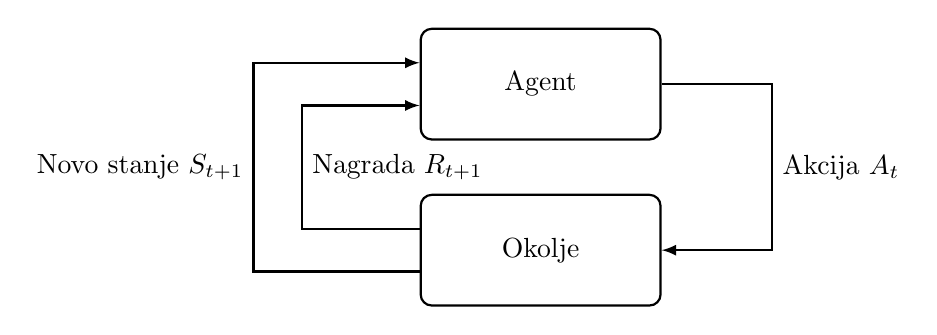
\begin{tikzpicture}[node distance = 6em, auto, thick]
    \node [block] (Agent) {Agent};
    \node [block, below of=Agent] (Okolje) {Okolje};

    \path [line] (Agent.0) --++ (4em,0em) |- node [near start]{Akcija $A_t$} (Okolje.0);
    \path [line] (Okolje.190) --++ (-6em,0em) |- node [near start] {Novo stanje  $S_{t+1}$} (Agent.170);
    \path [line] (Okolje.170) --++ (-4.25em,0em) |- node [near start, right] {Nagrada $R_{t+1}$} (Agent.190);
\end{tikzpicture}

\subsubsection{Raziskovanje in izkoriščanje}
Eden izmed glavnih problemov, s katerim se srečamo pri spodbujevalnem učenju, je problem 
raziskovanja in izkoriščanja. Ko se agent uči, začne dojemati, katere akcije ali pa kombinacije 
akcij mu pripeljejo nagrado. Ko to ugotovi, seveda lahko začne te akcije \textit{izkoriščati} 
in prejemati vso nagrado, ki akcijam pripada. Pri tem pa naletimo na problem. Agent lahko izkorišča te 
akcije in nikoli ne ugotovi, da neka druga akcija prinese še višjo nagrado; tega ne izve, ker ne
\textit{raziskuje}. Če pa samo raziskuje, pa nikoli ne izkoristi potencialnih nagrad, ki jih sreča, 
torej se ničesar ne nauči. 

Uravnoteženje raziskovanja in izkoriščanja je pomemben problem, a se izkaže, da ima dokaj enostavno
rešitev (ki deluje dovolj dobro). Spoznali jo bomo v madaljevanju.

Morda se nekaterim bralcem zdi, da smo zaenkrat preveč ">mahali z rokami"<. To je zato, ker želimo, 
da se do te točke razvije intuicija o predstavljenih pojmih. V nadaljevanju bomo do sedaj opisane 
stvari bolj formalizirali.


\subsection{Markovski proces odločanja}
Spomnimo se najprej procesa spodbujevalnega učenja in ga poskusimo opisati bolj formalno: 
imamo zaporedje časovnih korakov $t = 0, 1, 2, \dots$, ob katerih med sabo interaktirata agent 
in okolje. Ob koraku $t$ agent prejme od okolja stanje (oz. reprezentacijo stanja) $S_t \in 
\mathcal{S}$, kjer $\mathcal{S}$ označuje množico vseh stanj. Na podlagi stanja in strategije, 
ki jo ima, izbere akcijo $A_t \in \mathcal{A}(S_t)$, kjer $\mathcal{A}(S_t)$ predstavlja 
množico akcij, ki jih ima agent na voljo v stanju $S_t$. Rezultat te akcije je nagrada $R_{t+1} 
\in \mathcal{R}$, kjer $\mathcal{R} označuje mnoožico vseh nagrad$, in novo stanje $S_{t+1}$.

Čeprav se da vse opisane koncepte posplošiti na števne in celo neštevne množice stanj in akcij, 
se bomo mi omejili na končne množice. To je pri namiznih igrah dovolj.

\subsubsection{Markovska veriga}
Dogajanje pri spodbujevalnem učenju lahko v grobem opišemo z zaporedjem slučajnih spremenljivk $S_0,
S_1, \dots$ v diskretnem času, to je, s slučajnim procesom stanj $(S_t)_{t=0}^T$. Zato je pomembno, 
da si natančno pogledamo nekaj lastnosti, ki jih lahko pričakujemo. 

\begin{definicija}[Markovska veriga]
    Slučajni proces $(S_t)_{t=0}^T$ na končnem verjetnostnem prostoru 
    $(\Omega, \mathcal{F}, P)$ je \textbf{Markovska veriga} oz. \textbf{Markovski proces} (angl. 
    \textit{Markov chain}), če zanj velja Markovska lastnost
    $$
    P(S_{t+1} = s_{t+1}~|~S_{t} = s_{t}, \dots, S_0 = s_0) = P(S_{t+1} = s_{t+1}~|~S_{t} = s_{t}).
    $$
    Na kratko to \textit{prehodno verjetnost} označimo $p_{ss'} := P(S_{t+1} = s'~|~S_{t} = s)$.
    Opazimo, da lahko te verjetnsoti zložimo v matriko $\mathcal{P} := 
    [p_{ss'}]_{s,s'\in \mathcal{S} }$, ki ji pravimo \textit{prehodna matrika}.

    Zdaj Markovsko verigo predstavimo še na alternativni način: kot dvojico $(\mathcal{S}, 
    \mathcal{P})$, kjer je $\mathcal{P}$ zgoraj definirana prehodna matrika, $\mathcal{S}$ pa 
    množica vseh stanj.
\end{definicija}

Markovska lastnost pomeni, da je prihodnost neodvisna od preteklosti, če poznamo sedanjost. 
Spodbujevalno učenje se ukvarja predvsem s problemi, kjer to dejstvo drži. Tudi pri našem 
ciljnem problemu to načeloma velja: če pogledamo igralno ploščo na katerikoli točki, pogosto 
izvemo enako o trenutnem stanju, kot če bi opazovali igro od začetka.

\subsubsection{Markovski proces nagrajevanja}
Podoben koncept, ki se malo bolj približa dejanski situaciji v spodbujevalnem učenju, je
\textit{Markovski proces nagrajevanja}. Kot že ime morda namigne, je precej podoben Markovski 
verigi, le da v njem nastopajo \textit{nagrade}. 

\begin{definicija}[Markovski proces nagrajevanja]
    Pričakovani nagradi glede na stanje $s$ pravimo \textbf{nagradna funkcija} (angl. \textit{reward 
    function}) in jo označimo
    $$
    \mathcal{R}_s = E[R_{t+1}~|~S_{t} = s].
    $$
    Naboru $(\mathcal{S}, \mathcal{P}, \mathcal{R}, \gamma)$, za katerega velja
    \begin{itemize}
        \item $\mathcal{S}$ je (končna) množica stanj,
        \item $\mathcal{P}$ je prehodna matrika $\mathcal{P}_{ss'} = P(S_{t+1} = s'~|~S_{t} = s)$, 
        \item $\mathcal{R}$ je \textit{nagradna funkcija} 
                $\mathcal{R}_s = \mathrm{E}[R_{t+1}~|~S_{t} = s]$, 
        \item $\gamma \in [0,1]$ je \textit{diskontni faktor}, 
    \end{itemize}
    pravimo \textbf{Markovski proces nagrajevanja} (angl. \textit{Markov reward process}).
\end{definicija}

Od navadne Markovske verige se torej razlikuje samo v prisotnosti nagrad ob vsakem koraku. Če te 
nagrade postavimo na $R_t = 0$ za vsak $t$, dobimo navadno Markovsko verigo. Pomembna razlika je še 
prisotnost diskontnega faktorja $\gamma$. Če velja $\gamma < 1$, potem procesu pravimo \textit{
diskontirani Markovski proces nagrajevanja}.

Diskontiranje je motivirano iz različnih vidikov: po eni strani nam pomaga, da se v primeru 
cikličnih procesov izognemo neomejenim povračilom. Poleg tega pa je diskontiranje v mnogo pogledih 
naraven način za opis situacije: pogosto imamo raje nagrade, ki pridejo prej. Primer tega poznamo 
recimo iz ekonomije; denar, ki ga dobimo kasneje nam pomeni manj, kot tisti, ki ga dobimo takoj. 

Še vedno pa tovrsten proces ne opiše situacije, v kateri se znajdemo pri spodbujevalnem učenju, saj 
ne vsebuje koncepta akcij. Je pa že dovolj ">globok"<, da v njem lahko definiramo vrednostno 
funkcijo $v(s) = \mathrm{E} [G_t~|~S_t = s]$, ki je v tem primeru neodvisna od strategije $\pi$, 
saj strategija v tem modelu nima pomena. 

Za vrednostno funkcijo lahko izpeljemo rekurzivno enačbo, s pomočjo katere lahko ">rešimo"< Markovski
proces nagrajevanja. S tem mislimo, da vsakemu stanju dodelimo pravo vrednost:

\begin{align*}
    v(s) &= \mathrm{E} [G_t~|~S_t = s] \\
         &= \mathrm{E} [\sum_{k=0}^\infty \gamma^k R_{t + k + 1}~|~S_t = s] \\
         &= \mathrm{E} [R_{t+1} + \sum_{k=1}^\infty \gamma^k R_{t + k + 1}~|~S_t = s] \\
         &= \mathrm{E} [R_{t+1} + \gamma(\sum_{k=1}^\infty \gamma^{k-1} R_{t + k + 1})~|~S_t = s] \\
         &= \mathrm{E} [R_{t+1} + \gamma G_{t+1}~|~S_t = s] \\
         &= \mathrm{E} [R_{t+1} + \gamma v(S_{t+1})~|~S_t = s].
\end{align*}

Dobili smo torej 
$$
v(s) = \mathrm{E} [R_{t+1} + \gamma v(S_{t+1})~|~S_t = s]
$$
oziroma 
\begin{equation}\label{beMRP}
    v(s) = \mathcal{R}_s + \gamma \sum_{s' \in \mathcal{S}} \mathcal{P}_{ss'} v(s'),
\end{equation} 
kjer smo v drugi vrstici upoštevali aditivnost in idempotentnost pogojnega matematičnega upanja. 
Enačba \eqref{beMRP} je \textbf{Bellmanova enačba za Markovkse procese nagrajevanja}.

Ker se ukvarjamo s primerom, ko je stanj končno mnogo, recimo $n$, jih lahko brez škode za 
splošnost označimo kar $1, \dots, n$. Potem lahko Bellmanovo enačbo prepišemo v matrični obliki
\begin{align*}
    \begin{bmatrix}
        v(1) \\ 
        \vdots \\ 
        v(n)
    \end{bmatrix}
    &=
    \begin{bmatrix}
        \mathcal{R}_1 \\ 
        \vdots \\ 
        \mathcal{R}_n 
    \end{bmatrix}
    + \gamma
    \begin{bmatrix}
        \mathcal{P}_{11} \dots \mathcal{P}_{1n} \\ 
        \vdots \\ 
        \mathcal{P}_{n1} \dots \mathcal{P}_{nn}
    \end{bmatrix}
    \begin{bmatrix}
        v(1) \\ 
        \vdots \\ 
        v(n)
    \end{bmatrix} \\
    \intertext{ali krajše}
    v &= \mathcal{R} + \gamma \mathcal{P}v.
\end{align*}
Opazimo, da je to \textit{linearna} enačba in da v splošnem eksplicitno rešitev: 
\begin{align*}
    v &= \mathcal{R} + \gamma \mathcal{P}v \\
    (I - \gamma \mathcal{P}) v &= \mathcal{R} \\
    v &= (I - \gamma \mathcal{P})^{-1} \mathcal{R}.
\end{align*}
Ta rešitev predpostavlja obrnljivost matrike $(I - \gamma \mathcal{P})$ in računanje njenega 
inverza, kar zahteva $O(n^3)$ operacij, zato je smiselna samo za majhne procese. Za večje 
obstajajo iterativni algoritmi in metode, nekatere izmed njih bomo spoznali v naslednjem odseku.

TA DEL LAHKO MATEMATIZIRAŠ - ENOLIČNOST REŠITEV

\subsubsection{Markovski proces odločanja}
Kot ime že nakazuje, \textit{Markovski proces odločanja (MDP)} razširja koncept procesa nagrajevanja 
z dodatkom odločanja - akcij. S tem dodatkom imamo v popolnosti opisan problem spodbujevalnega 
učenja: opisujemo torej nek proces, kjer ima agent možnost odločanja, izid pa je vsaj delno slučajen 
in odvisen od okolja. 

\begin{opomba}
    Ker v Markovskem procesu odločanja nastopajo (in imajo poglavitno) vlogo akcije, seveda pomembno 
    vplivajo na nagradno funkcijo, zato moramo ta koncept ustrezno prilagoditi:
    $$
    \mathcal{R}_s^a = E[R_{t+1}~|~S_{t} = s, A_t = a].
    $$
\end{opomba}

\begin{definicija}[Markovski proces odločanja]
    Naboru $(\mathcal{S}, \mathcal{A}, \mathcal{P}, \mathcal{R}, \gamma)$, za katerega velja
    \begin{itemize}
        \item $\mathcal{S}$ je (končna) množica stanj,
        \item $\mathcal{A}$ je (končna) množica akcij, 
        \item $\mathcal{P}$ je prehodna matrika $\mathcal{P}_{ss'}^a = P(S_{t+1} = s'~|~
                S_t = s, A_t = a)$, 
        \item $\mathcal{R}$ je \textit{nagradna funkcija} 
                $\mathcal{R}_s^a = \mathrm{E}[R_{t+1}~|~S_{t} = s, A_t = a]$, 
        \item $\gamma \in [0,1]$ je \textit{diskontni faktor}, 
    \end{itemize}
    pravimo \textbf{Markovski proces odločanja} (angl. \textit{Markov decision process}).
\end{definicija}

Prehodna matrika in nagradna funkcija sta sedaj seveda odvisni tudi od akcije. V kontekstu MDP-jev
lahko sedaj formalno definiramo strategijo agenta $\pi$, ki je zahvaljujoč Markovski lastnosti 
odvisna od enega stanja in ne od celotne zgodovine procesa. Definiramo tudi vrednostno funkcijo 
stanja $v_{\pi}(s)$ in vrednostno funkcijo akcije $q_{\pi}(s, a)$. Njihove definicije se ne 
spremenijo, so pa sedaj formalno umeščene v model.

Opazimo tudi, da je v MDP-ju pri fiksni strategiji $\pi$ zaporedje oz. proces stanj $S_1, S_2, 
\dots$ Markovska veriga $(\mathcal{S}, \mathcal{P}^\pi)$. Če v zaporedje stanj pomešamo še nagrade, 
torej $S_1, R_2, S_2, R_3, \dots$, dobimo Markovski proces nagrajevanja $(\mathcal{S}, 
\mathcal{P}^\pi, \mathcal{R}^\pi, \gamma)$, kjer smo označili

\begin{align*}
    \mathcal{P}^\pi &= \sum_{a \in \mathcal{A}} \pi(a|s) \mathcal{P}_{ss'}^a \\
    \mathcal{R}^\pi &= \sum_{a \in \mathcal{A}} \pi(a|s) \mathcal{R}_{s}^a. 
    \end{align*}

\begin{opomba}
    Morda je nekatere bralce zbodlo, da v zaporedju stanj in nagrad $S_1$ ne sledi $R_1$, temveč 
    $R_2$. Za tako notacijo smo se odločili, da poudarimo, da okolje agentu sočasno poda $S_2$ in 
    $R_2$, glede na stanje $S_1$ pa se agent odloča o akciji $A_1$.
\end{opomba}

MDP-ji so splošna orodja za obravnavo stohastičnih procesov, ki vključujejo odločitve v diskretnem 
času. Njihov utemeljitelj je Richard Bellman, ki je znan predvsem po izumu dinamičnega 
programiranja, zato morda ni presenetljivo, da nam prav dinamično programiranje poda osnovo za 
njihovo reševanje.
Kot pri procesih nagrajevanja, lahko tudi tu izpeljemo Bellmanovo enačbo. Najprej zapišemo 
rekurzivni zvezi za vrednostni funkciji stanja in akcije: 

\begin{align*}
    v_\pi(s) &= \mathrm{E} [R_{t+1} + \gamma v_\pi(S_{t+1})~|~S_t = s], \\
    q_\pi(s, a) &= \mathrm{E} [R_{t+1} + \gamma q_\pi(S_{t+1}, A_{t+1})~|~S_t = s, A_t = a].
\end{align*}
Opazimo, da $v_\pi$ in $q_\pi$ povezujta zvezi

\begin{align*}
    v_\pi(s) &= \sum_{a \in \mathcal{A}} \pi(a|s)q_\pi(s, a), \\
    q_\pi(s, a) &= \mathcal{R}_s^a + \gamma \sum_{s' \in \mathcal{S}} \mathcal{P}_{ss'}^a v_\pi(s').
\end{align*}
Če zvezi združimo, dobimo

\begin{align}
    v_\pi(s) &= \sum_{a \in \mathcal{A}} \pi(a|s) \left[\mathcal{R}_s^a + 
    \gamma \sum_{s' \in \mathcal{S}} \mathcal{P}_{ss'}^a v_\pi(s') \right], \label{bepMDP} \\
    q_\pi(s, a) &= \mathcal{R}_s^a + \gamma \sum_{s' \in \mathcal{S}} 
    \mathcal{P}_{ss'}^a \left[\sum_{a' \in \mathcal{A}} \pi(a'|s')q_\pi(s', a') \right].
\end{align}
Enačbo \eqref{bepMDP} imenujemo \textbf{Bellmanova enačba pričakovanja} (angl. \textit{Bellman 
expectation equation}), ki ima ponovno matrično obliko in eksplicitno (ENOLIČNO - ZAKAJ, TU 
DODATNA RAZLAGA) rešitev: 
\begin{align*}
    v_\pi &= \mathcal{R}^\pi + \gamma \mathcal{P}^\pi v_\pi \\
    v_\pi &= (I - \gamma \mathcal{P}^\pi)^{-1} \mathcal{R}^\pi
\end{align*}

Ta enačba je sicer pomembna, a nas najbolj zanima ">rešitev"< MDP-ja. Želimo namreč najti optimalno 
strategijo. Pri tem nam pomaga naslednje: 

\begin{definicija}
    ~
    \begin{itemize}
        \item \textbf{Optimalna vrednostna funkcija stanja} (angl. \textit{optimal state-value 
                function}) $v_*(s)$ je največja med vsemi vrednostnimi funkcijami stanj
                $$
                v_*(s) = \max_\pi v_\pi(s).
                $$
        \item \textbf{Optimalna vrednostna funkcija akcije} (angl. \textit{optimal action-value 
                function}) $q_*(s, a)$ je največja med vsemi vrednostnimi funkcijami akcij
                $$
                q_*(s, a) = \max_\pi q_\pi(s, a).
                $$
        \item Na množici vseh možnih strategij $\Pi$ definiramo delno urejenost na naslednji način:
                $$
                \pi \geq \pi', \medspace \text{če } v_\pi(s) \geq v_{\pi'}(s) ~ \forall s. 
                $$
                Če za strategiji velja kot zgoraj, pravimo, da je $\pi$ \textit{boljša ali enaka} 
                kot $\pi'$.
    \end{itemize}
\end{definicija}
Sedaj lahko uporabimo naslenji izrek.

\begin{izrek}\label{optim}
    Za vsak Markovski proces odločanja velja: 
    \begin{itemize}
        \item Obstaja \textit{optimalna} strategija $\pi_*$, ki je boljša ali enaka kot vse ostale 
                strategije; $\pi_* \geq \pi \text{ } \forall \pi \in \Pi$. 
        
        \item Vedno obstaja \textit{deterministična} optimalna strategija. PREJ RAZLOŽI NATANČNO 
                STRATEGIJE
        \item Vse optimalne strategije določajo optimalno vrednostno funkcijo stanja in optimalno 
                vrednostno funkcijo akcije; 
                \begin{align*}
                    v_{\pi*}(s) &= v_*(s) \\
                    q_{\pi*}(s, a) &= q_*(s, a).
                \end{align*}
    \end{itemize} 
\end{izrek}

OPOMBA: SKLIC NA DOKAZ

Izrek nam pove, da če poznamo $q_*(s, a)$, poznamo tudi optimalno deterministično strategijo, 
ki jo dobimo kot $\pi_*(a|s) = \mathbbm{1} (a =\text{arg}\max_{a \in \mathcal{A}} q_*(s, a))$.

Podobno kot za poljubne vrednostne funkcije, lahko tudi za optimalne vrednostne funkcije 
izpeljemo Bellmanovo enačbo, ki jo sedaj imenujemo \textbf{Bellmanova enačba optimalnosti} (angl. 
\textit{Bellman optimality equation}). Sprva opazimo zvezi med $q_*$ in $v_*$:

IZPELJI TI DVE ZVEZI

\begin{align*}
    v_*(s) &= \max_a q_*(s, a), \\
    q_*(s, a) &= \mathcal{R}_s^a + \gamma \sum_{s' \in \mathcal{S}} \mathcal{P}_{ss'}^a v_*(s).
\end{align*}
Ti zvezi nato vstavimo eno v drugo, in dobimo enačbi: 

\begin{align}\label{beo}
    v_*(s) &= \max_a \mathcal{R}_s^a + \gamma \sum_{s' \in \mathcal{S}} \mathcal{P}_{ss'}^a v_*(s), \\
    q_*(s, a) &= \mathcal{R}_s^a + 
                \gamma \sum_{s' \in \mathcal{S}} \mathcal{P}_{ss'}^a \max_{a'} q_*(s', a').
\end{align}
Opazimo, da sta enačbi tokrat nelinearni, kar močno oteži direktno reševanje. Na srečo pa tudi 
v tem primeru pridejo prav metode iz naslednjega odseka.

\section{Algoritmi pri spodbujevalnem učenju}
Algoritmov za reševanje MDP-jev je precej. Mi se bomo omejili predvsem na algoritme, ki se učijo 
prek vrednostne funkcije in izhajajo iz dinamičnega programiranja, a naj na tem mestu omenimo, 
da obstajajo tudi algoritmi, ki posodabljajo strategijo neposredno (MOGOČE KAKŠEN REFERENCE ALI 
PA KEJ).

Izjemnega pomena pri reševanju je tudi dejstvo, ali je znana matrika $\mathcal{P}$ in nagradna 
funkcija $\mathcal{R_s^a}$. Izkaže se, da je večina problemov takih, da ti dve stvari nista znani. 
Eden izmed takih problemov je tudi igranje namiznih iger -- ne poznamo strategije našega nasprotnika, 
zato ne poznamo verjetnosti prehodov med stanji.

Poleg tega naj na tem mestu omenimo, da reševanju celotnega problema spodbujevalnega učenja 
pravimo \textbf{načrtovanje} (angl. \textit{planning}), le-ta pa se deli na dve stopnji: 

\begin{itemize}
    \item \textbf{Napovedovanje} - pri tem podproblemu podamo nek MDP in strategijo, algoritem nam 
            vrne vrednostno funkcijo stanja (glede na strategijo).   
    \item \textbf{Upravljanje} - to je bolj poln problem: podan je MDP, algoritem pa nam vrne 
            optimalno vrednostno funkcijo in optimalno strategijo.
\end{itemize}

\subsection{Dinamično programiranje - reševanje poznanih MDP-jev}
Dinamično programiranje je optimizacijska metoda, ki deluje na principu deljenja velikega problema 
na manjše prekrivajoče podprobleme. V jedru reševanja je \textbf{Bellmanova enačba}, ki opisuje 
odnos med vrednostmi podproblemov in vrednostjo glavnega problema. Ker je idejo dinamičnega 
programiranja (DP) in MDP-jev dobil Bellman ob istem času, je naravno, da je DP metoda, ki je 
prilagojena prav situaciji v MDP-ju.

Problem mora v splošnem zadoščati dvema lastnostima, da je zanj primerno reševanje z dinamičnim 
programiranjem. Prvi pravimo \textbf{lastnost optimalne podstrukture}, ki pravi, da lahko problem 
razstavimo na podprobleme in rešitve podproblemov lahko potem sestavimo nazaj v rešitev celotnega 
problema. Druga pomembna lastnost pa so \textbf{prekrivajoči podproblemi}, ki implicira, da lahko 
že poznane rešitve podproblemov večkrat uporabimo.

Opazimo, da obe lastnosti veljata za MDP-je; Bellmanova enačba, nam razdeli problem na 
podprobleme, vrednostna funkcija pa hrani in ponovno uporablja rešitve. Lastnosti veljata tudi 
za MRP-je in tudi metode, ki jih bomo spoznali so aplikativne na njih, a mi se bomo posvetili 
predvsem procesom odločanja.

(MORDA BOLJ FORMALNO O BELLMANOVIH ENAČBAH - NI TREBA?)

\subsubsection{Iterativno ocenjevanje strategije}
Algoritem deluje na MDP-ju, katerega prehodna matrika je znan podatek. Poleg tega potrebuje tudi 
fiksno strategijo $\pi$. Algoritem torej rešuje zgorlj parcialni problem, to je problem 
napovedovanja. V ozadju je glavna ideja Bellmanova enačba pričakovanja, z njo na vsakem koraku 
posodobimo $v_k(s)$ v $v_{k+1}(s)$ s pomočjo $v(s')$, kjer je $s'$
naslednje stanje od $s$. Enačba iteracije se potem glasi 
\begin{align*}
    v_{k+1}(s) &= \sum_{a \in \mathcal{A}} \pi(a|s) \left[ \mathcal{R}_s^a + 
        \gamma \sum_{s' \in \mathcal{S}} \mathcal{P}_{ss'}^a v_k(s') \right] \text{ ali na kratko}\\
    v_{k+1} &= \mathcal{R}^\pi + \gamma \mathcal{P}^\pi v_k.
\end{align*}

\begin{izrek}
    Iterativno ocenjevanje strategije konvergira proti vrednostni funkciji, ki jo določa strategija 
    $\pi$.
\end{izrek}

\begin{proof}
    Pokazali bomo, da iz iteracije lahko pridobimo skrčitev, iz izrekov o fiksni točki potem sledi 
    naš rezultat (MOGOČE DEJMO NAVEST IZREK? - BANACH, CONTRACTION MAPPING) - LAHKO SKLIC NA 
    LITERATURO.

    Definiramo \textbf{Bellmanov operator pričakovanja} kot 
    $$
    T_\pi(v) = \mathcal{R}_\pi + \gamma \mathcal{P}_\pi v.
    $$

    POVEŠ KAKO JE DEFINIRANA OPERATORSKA NESKONČNA NORMA
    Naj bosta $u$ in $v$ vrednostni funkciji. Potem je zgornji operator skrčitev glede na neskončno 
    normo: 
    \begin{align*}
        ||T_\pi(v) - T_\pi(u)||_\infty &= ||\mathcal{R}_\pi + \gamma \mathcal{P}_\pi v - 
                                            \mathcal{R}_\pi + \gamma \mathcal{P}_\pi u||_\infty \\  
        &= ||\gamma \mathcal{P}_\pi (v - u)||_\infty \\
        &\leq ||\gamma \mathcal{P}_\pi||_\infty ||v - u||_\infty \\
        &\leq \gamma ||v - u||_\infty,
    \end{align*}
    kjer smo upoštevali, da velja $||\mathcal{P}_\pi||_\infty \leq 1$, saj so elementi 
    $\mathcal{P}_\pi$ verjetnosti.

\end{proof}

S tem procesom tako res dobimo vrednostno funkcijo, ki jo določa strategija, a strategija je 
statična; to reši problem napovedovanja. 

Da rešimo problem upravljanja, uporabimo enostavno idejo: strategijo izboljšamo \textbf{požrešno}. 
To pomeni, da izberemo tako akcijo, ki nas pripelje v stanje, ki je dosegljivo in ima trenutno 
največjo vrednost $v_\pi$.

\subsubsection{Iteracija strategije}
Algoritem, ki ga dobimo s tem, da združimo iterativno ocenjevanje strategije in požrešno izboljšavo 
strategije, imenujemo iteracija strategije (angl. \textit{policy iteration}). S tem algoritmom 
lahko sedaj rešimo problem upravljanja in s tem celoten problem poznanega MDP-ja. 

\begin{trditev}
    Iteracija strategije vedno konvergira k optimalni strategiji $\pi_*$.
\end{trditev}

\begin{proof}
    Ukvarjali se bomo samo z determinističnimi strategijami, saj so zaradi požrešne izbire 
    strategije le-te vedno deterministične, razen začetne. Ker je izbira začetne strategije za 
    trditev nepomembna, lahko izberemo neko naključno deterministično strategijo $a = \pi(s)$.

    Požrešno vedenje zdaj za nas pomeni, da vzamemo $\pi'(s) = 
    \text{arg}\max_{a \in \mathcal{A}} q_\pi(s, a)$. To očitno izboljša vrednost za vsako stanje 
    $$
    q_\pi(s, \pi'(s)) = \max_{a \in \mathcal{A}} q_\pi(s, a) \geq q_\pi(s, \pi(s)) = v_\pi(s).
    $$
    Posledično izboljša tudi vrednostno funkcijo: 
    \begin{align*}
        v_\pi(s) &\leq q_\pi(s, \pi'(s)) = \mathrm{E}_{\pi'} [R_{t+1} + 
            \gamma v_\pi(S_{t+1})~|~S_t = s] \\
        &\leq \mathrm{E}_{\pi'} [R_{t+1} + \gamma q_\pi(S_{t+1} \pi'(S_{t+1}))~|~S_t = s] \\
        &\leq \mathrm{E}_{\pi'} [R_{t+1} + \gamma R_{t+2} + 
            \gamma^2 q_\pi(S_{t+2} \pi'(S_{t+2}))~|~S_t = s] \\
        &\leq \mathrm{E}_{\pi'} [R_{t+1} + \gamma R_{t+2} + \dots~|~S_t = s] = v_{\pi'}(s).
    \end{align*}

Če vrednost preneha rasti, dobimo 
$$
q_\pi(s, \pi'(s)) = \max_{a \in \mathcal{A}} q_\pi(s, a) = q_\pi(s, \pi(s)) = v_\pi(s).
$$
To se zgodi, saj zaradi končnih nagrad tudi vrednostne funkcije zavzemajo končne vrednosti. 
Potem opazimo, da je zaradi $v_\pi(s) = \max_{a \in \mathcal{A}} q_\pi(s, a)$ zadoščeno Bellmanovi 
enačbi optimalnosti in zato po izreku \ref{optim} velja $v_\pi(s) = 
v_*(s) \text{ } \forall s \in \mathcal{S}$, torej je $\pi$ optimalna strategija.
\end{proof}

\subsubsection{Iteracija vrednosti}
K problemu lahko pristopimo tudi neposredno prek Bellmanove enačbe optimalnosti in se s tem 
izognemo neposredni uporabi strategije, vseeno pa rešimo problem upravljanja. Ideja je podobna kot 
pri iterativnem ocenjevanju strategije, le da imamo drugačno enačbo za iteracijo: 
\begin{align*}
    v_{k+1}(s) &= \max_{a \in \mathcal{A}} \left[ \mathcal{R}_s^a + 
        \gamma \sum_{s' \in \mathcal{S}} \mathcal{P}_{ss'}^a v_k(s') \right] \\
    \intertext{oziroma}
    v_{k+1} &= \max_{a \in \mathcal{A}} \mathcal{R}^a + \gamma \mathcal{P}^a v_k.
\end{align*}
Podobno kot pri iterativnem ocenjevanju strategije pokažemo, da zgornja iteracija konvergira k 
$v_*$.

\subsubsection{Časovna zahtevnost}
Za korak obeh iteracij je potrebnih $O(mn^2)$ operacij, kjer je $m$ število akcij in $n$ število 
stanj. Popolnoma enake algoritme lahko uporabimo za iteracijo $q_\pi(s, a)$ oz. $q_*(s, a)$, le 
da sedaj pridemo do časovne zahtevnosti $O(m^2n^2)$.

\subsubsection{a sm js pozabu na generalised policy evaluation}

\subsection{Monte Carlo}
Do sedaj smo se ukvarjali s poznanim MDP-jem, kar pa ni naš končen cilj. V nadaljevanju se bomo 
posvetili nepoznanim. Metode, ki jih bomo spoznali so tako bolj splošno aplikativne, svoje 
bistvo pa črpajo pri do sedaj poznanem.

Prva taka metoda je Monte Carlo. Spopada se s problemom napovedovanja z dodatno izboljšavo, da 
ne rabi poznati matrike $\mathcal{P}$. Potrebujemo pa strategijo $\pi$, na podlagi katere opazujemo 
epizode dogajanja. Ideja delovanja je, da se namesto na direktno računanje pričakovanega povračila
$G_t = \sum_{k=0}^\infty \gamma^k R_{t + k + 1}$, osredotočimo na računanje \textit{empiričnega} 
povračila. To storimo tako, da za vsako stanje $s$ definiramo števec $N(s)$, ki beleži, kolikokrat 
je bilo stanje obiskano. Ta števec ne beleži zgolj obiskov znotraj epizode, temveč skozi celoten 
proces učenja. Za vsako stanje hranimo še $S(s)$, ki mu ob vsakem obisku prištejemo pričakovano 
povračilo. To seveda pomeni, da se vrednost stanja ne more posodobiti takoj po obisku, ampak šele 
ob koncu epizode, ko je $G_t$ znan. Po koncu učenja enostavno za vsako stanje delimo $S(s)$ z $N(s)$
in tako dobimo vzorčno povprečje za dejanski $v(s)$.

\begin{itemize}
    \item Ob vsakem (ali samo prvem) obisku stanja $s$: 
        \begin{align*}
            N(s) &\leftarrow N(s) + 1 \\
            S(s) &\leftarrow S(s) + G_t.
        \end{align*}
    \item Po zadostni količini epizod (ob koncu učenja): 
        $$
        V(s) \leftarrow S(s) / N(s)
        $$
\end{itemize}
TOLE MALO BOLJ RAZDELAJ - MONTE CARLO IMA KVADRATIČNO KONVERGENCO, SUTTON BARTO
Opazimo, da vrednost $V(s)$ konvergira proti $v_\pi(s)$, ko gre $N(s) \rightarrow \infty$ po 
krepkem zakonu velikih števil. Opazimo tudi, da metoda deluje samo za probleme, ki imajo končne 
epizode, saj šele takrat lahko poznamo $G_t$. Če za vsako stanje $s$ hranimo $N(s)$ in $S(s)$, 
tako dobimo oceno za $v_\pi(s)$ za vsak $s \in \mathcal{S}$.

Prostorsko zahtevnost lahko izboljšamo, če upoštevamo, da povprečje $\mu$ nekega zaporedja slučajnih 
spremenljivk $X_1, X_2, \dots$ izračunamo inkrementalno:
\begin{align*}
    \mu_k &= \frac{1}{k} \sum_{i = 1}^k X_i \\
        &= \frac{1}{k} \left[X_k + \sum_{i = 1}^{k-1} X_i \right] \\
        &= \frac{1}{k} \left[X_k + (k-1) \mu_{k-1} \right] \\
        &= \mu_{k-1} + \frac{1}{k} \left(X_k - \mu_{k-1} \right).
\end{align*}

Na podlagi te zveze lahko implementiramo inkrementalni Monte Carlo, tako da po končani epizodi 
za vsako stanje $S_t$ s povračilom $G_t$ posodobimo (ODLOČI SE ZA $S_t$ ALI s): 

\begin{align*}
    N(S_t) &\leftarrow N(S_t) + 1, \\
    V(S_t) &\leftarrow V(S_t) + \frac{1}{N(S_t)} (G_t - V(S_t)).
\end{align*}
Izkaže se, da lahko zgornje še malo posplošimo in uporabimo

\begin{equation}\label{mc}
    V(S_t) \leftarrow V(S_t) + \alpha (G_t - V(S_t)),
\end{equation}
kjer $\alpha$ imenujemo \textbf{velikost koraka} oz. \textbf{hitrost učenja} (angl. 
\textit{learning rate}). Posodobitveno pravilo \eqref{mc} je konkreten primer bistvene ideje 
spodbujevalnega učenja prek vrednostne funkcije. Vsi ostali algoritmi nam dajo pravilo podobne 
oblike: 
\begin{equation}\label{osnova}
    \textit{nova ocena} \leftarrow \textit{stara ocena} + \textit{korak } 
    (\textit{tarča} - \textit{stara ocena}).
\end{equation}

\subsection{Algoritem $TD(0)$}
V spodbujevalnem učenju obstaja skupina algoritmov, ki se imenujejo \textbf{algoritmi učenja s 
časovno razliko} (angl. \textit{temporal-difference learning}). Delujejo v podobnih pogojih kot 
Monte Carlo in tudi dosegajo enak cilj. Pomembna razlika je, da ne potrebujejo povračila pri 
posodobitvi. Delujejo lahko tudi v sistemih, ki se ne delijo na epizode oz. ne potrebujejo 
končanih epizod za svoje delovanje.

Najpreprostejši algoritem učenja s časovno razliko je $TD(0)$. Ideja je, da v stanju ocenimo
povračilo kot $G_t \approx R_{t+1} + \gamma V(S_{t+1}).$ To potem uporabimo za \textit{tarčo}
v pravilu \eqref{osnova}. To nam da pravilo
\begin{equation}
    V(S_t) \leftarrow V(S_t) + \alpha (R_{t+1} + \gamma V(S_{t+1}) - V(S_t)).
\end{equation}
Iz tega zelo hitro ugotovimo, od kod pride poimenovanje. Algoritem za svoje posodabljanje uporablja 
podatek iz naslednjega trenutka - torej se uči s časovno razliko. Pomembno je omeniti tudi, da  za 
učenje uporablja oceno, torej ocenjuje na podalgi ocene. Temu pravimo \textit{zankanje} (angl. 
\textit{bootstrapping}).

\subsubsection{Primerjava z Monte Carlo}
\begin{itemize}
    \item Tarča pri MC je nepristranska ocena $v_\pi(S_t)$, medtem ko je pri TD(0) tarča 
    pristranska ocena. Ta prednost MC je uravnotežena s tem, da ima TD(0) tarča nižjo varianco, 
    saj je odvisna od ene same slučajne spremenljivke, medtem ko je pri MC odvisna od mnogih 
    slučajnih dogodkov.
    
    \item Prav tako je pomembna razlika v dejstvu, da MC nujno rabi popolne epizode in se lahko
    izvede le po končani epizodi, TD(0) pa se lahko uči sproti (angl. \textit{online}) in sploh 
    ne potrebuje končnih epizod.

    \item Razlika je tudi v tem, kam konvergirata algoritma, če imamo na voljo samo končno 
    količino epizod. Naj $K$ označuje število epizod in $k$ nakazuje, v kateri epizodi smo. Potem 
    MC konvergira k rešitvi z minimalno povprečno kvadratno napako (MSE) 
    $$
    \sum_{k=1}^K \sum_{t=1}^{T_k} (G_t^k - V(s_t^k))^2,
    $$
    torej se najbolje prilega opazovanim povračilom. TD(0) pa konvergira k rešitvi modela največjega 
    verjetja Markova; to je rešitev MDP-ja, ki se najbolje prilega podatkom. Dobimo torej naslednji 
    cenilki: (TO SI ŠE POGLEJ)
    \begin{align*}
        \hat{\mathcal{P}}_{ss'}^a &= \frac{1}{N(s, a)} \sum_{k=1}^K \sum_{t=1}^{T_k} 
                \mathbbm{1}(s_t^k, a_t^k, s_{t+1}^k = s, a, s') \\
        \hat{\mathcal{R}}_{s}^a &= \frac{1}{N(s, a)} \sum_{k=1}^K \sum_{t=1}^{T_k} 
                \mathbbm{1}(s_t^k, a_t^k = s, a)r_t^k
    \end{align*}

    \item Zadnja pomembna razlika je, da TD izrabi Markovsko lastnost, medtem ko je MC ne. Zato je 
    vsaj v teoriji TD veliko bolj učinkovit v MDP-jih.
\end{itemize}

\begin{zgled}[Ti si sodnik - IZ SUTTON BARTO UČBENIKA]
    Recimo, da imamo na voljo za učenje naslednjih 8 epizod: 
    A $0$, B, $0$;
    B $1$;
    B $1$;
    B $1$;
    B $1$;
    B $1$;
    B $1$;
    B $0$

    To pomeni recimo, da smo prvo epizodo začeli v stanju A, nato dobili nagrado $0$ in prešli v 
    stanje B, kjer smo ponovno dobili nagrado $0$, tu pa se je epizoda končala. Če bi se učili 
    samo iz teh osmih epizod, bi se verjetno vsi strinjali, da je $V(B) = 3/4$, saj je v šestih
    opažanjih B zavzel vrednost $1$, v dveh pa $0$. Z nami se strinjata tudi $TD(0)$ in $MC$. 

    Razlike se začenjo pri stanju A. $MC$, ki minimizira povprečno kvadratno napako in zato ob 
    enem opažanju A, ki je dal nagrado $0$, enostavno reče $V(A) = 0$ - to ima celo ničelno 
    napako glede na podatke. 

    $TD(0)$ pa pristopi nekoliko drugače. Vedno, ko smo opazili A, smo potem takoj opazili tudi B
    (vmes smo prejeli nagrado $0$), zato je smiselno, da je vrednost stanja A enaka vrednosti 
    stanja B, tj. $V(A) = 3/4$. V tem pristopu smo si pomagali tako, da smo problem modelirali kot 
    markovski proces.
\end{zgled}

\subsection{$TD(\lambda)$}
Algoritma, ki smo ju spoznali do sedaj mogoče na prvi pogled nista najbolj podobna, a bomo kmalu 
videli, da pripadata isti družini algoritmov. V ta namen si poglejmo povračila, ki gledajo $n$-
korakov v prihodnost. Tarča se primerno prilagodi v: 
$$
G_t^{(n)} = R_{t+1} + \dots + \gamma^{n-1} R_{t+n} + \gamma^n V(S_{t+1}).
$$
To tarčo lahko uporabimo v pravilu \eqref{osnova}. S tem dobimo algoritem, ki se imenuje \textit{
učenje s časovno razliko z $n$ koraki}. Opazimo tudi, da z večanjem $n$ proti neskončno pridemo na 
neki točki do že znanega MC pravila. Hitro tudi vidimo, da to pravilo sicer res poveže $TD(0)$ in 
MC, a ne predstavlja nobene bistvene izboljšave. Pojavi pa se še dodaten problem. Če smo v času, ki
je manj kot $n$ korakov stran od konca epizode, ne moremo porabiti celotnega $G_t^{(n)}$. V tem 
primeru enostavno vzamemo toliko korakov naprej, kot nam čas dopušča. To pomeni, da se vedemo enako 
kot pri MC algoritmu.

Nadgradnjo algoritma nam da dejstvo, da lahko skupaj združujemo podatke iz različnih časov prek 
tega, da povprečimo $G_t^{(n)}$ za različne $n$. V nadaljevanju bomo pogledali, kako združimo 
podatke iz vseh časov, ki nastopijo. Najti moramo ustrezne uteži, ki se seštejejo v ena in so 
smiselne glede na obravnavan problem. Primernega kandidata sta našla CITIRAJ ITD ITD, in sicer:
$$
G_t^\lambda = (1 - \lambda) \sum_{n=1}^\infty \lambda^{(n-1)} G_t^{(n)}.
$$

Od tu takoj sledi algoritem \textbf{$TD(\lambda)$ s pogledom naprej} (angl. \textit{forward-view 
$TD(\lambda)$}). To poimenovanje izhaja iz dejstva, da kot MC, tudi ta algoritem potrebuje znanje
prihodnosti, da posodobi vrednsoti; z drugimi besedami, uči se lahko samo iz popolnih epizod.

Čeprav je teoretično zanimiv algoritem, je v praksi veliko bolj uporaben algoritem, ki ne potrebuje
vedenja o prihodnosti in se tako lahko uči \textit{">online"<}. Izkaže se, da je zgornji algoritem 
mogoče popraviti in ga spremeniti v bolj praktično verzijo.

ZAKAJ JE TO POVEZAVA MED TD(0) IN MC!!!!!

\subsubsection{Sledi upravičenosti (angl. \textit{Eligibility traces})}
Prek tega koncepta lahko spremenimo algoritem tako, da se lahko uči po vsaki potezi sproti. Ideja 
je, da za vsako stanje hranimo njegovo sled upravičenosti. Konceptualno to za nas pomeni, da sproti 
ugotavljamo, kako zasluženo je stanje za morebitno nagrado - koliko je pripomoglo k njeni 
pridobitvi.

Praktično pa je sled upravičenosti slučajna spremenljivka $E_t: \mathcal{S} \rightarrow \mathbb{R}^+$. 
Pri sledeh sta pomembni dve stvari: \textbf{čas}, ki je pretekel od obiska in \textbf{pogostost} 
obiska stanja. Sledi upravičenosti združijo oboje. Za stanje tako lahko napišemo enostavno enačbo, 
kjer je z $E_t(s)$ označena sled v času $t$ za stanje $s$:
\begin{align*}
    E_0(s) &= 0 \\
    E_t(s) &= \gamma \lambda E_{t-1}(s) + \mathbbm{1}(S_t = s),
\end{align*}
kjer sta $\gamma$ in $\lambda$ že poznana parametra. Pomensko torej sled propada z oddaljevanjem 
od obiska $s$, v primeru, da je $s$ ponovno obiskan, pa skoči za $1$. S tem lahko torej dodelimo 
nagrade oz. kazni samo tistim stanjem, ki to zaslužijo. V tem pogledu je to res osnovni mehanizem 
za dodeljevanje nagrad, ko smo dodatno vezani še na čas.

S tem novim konceptom lahko posodobimo naš algoritem. Če označimo napako kot $\delta_t = R_{t+1} + 
\gamma V(S_{t+1}) - V(S_t)$, potem zapišemo: 
\begin{equation}\label{TDlambda}
    V(s) \leftarrow V(s) + \alpha \delta_t E_t(s).
\end{equation}
Poleg zgoraj definiranih sledi, ki jim pravimo \textit{akumulativne sledi}, obstajata še dve 
alternativi:

\begin{itemize}
    \item \textit{Nadomeščujoče sledi}, ki so podobne akumulativnim, le da ob obisku ni skoka za 
            $1$, pač pa skok za $1$, drugače pa imajo enako lastnost propadanja kot akumulativne. 
    \item \textit{Nizozemske sledi}, ki jih definiramo $E_t(s) = (1 - \alpha) \gamma \lambda 
            E_{t-1}(s) + \mathbbm{1}(S_t = s)$. Torej podobno kot akumulativne, le da so dodatno 
            pomnožene z $(1 - \alpha)$. Ideja je, da s tem dodatnim členom dobimo sled, ki je med 
            akumulativno in nadomeščujočo.
\end{itemize}

V zgornji formulaciji pravila $TD(\lambda)$ je tudi bolj očitno, zakaj ta algoritem poveže $TD(0)$ 
in $MC$:

\begin{itemize}
    \item Če je $\lambda = 0$, potem velja $E_t(s) = \mathbbm{1}(S_t = s)$, torej se posodobi samo
            trenutno stanje: $V(S_t) \leftarrow V(s_t) + \alpha \delta_t$, kar pa je natančno 
            posodobitev pri $TD(0)$.
    \item Za $TD(1)$ pa je za nagrado zaslužno vsako stanje, tako kot pri $MC$. Pravo ekvivalenco 
            nam pomaga videti naslednji izrek.
\end{itemize}

\begin{izrek}
    Vsota posodobitev vrednosti ob koncu epizode je enaka za $TD(\lambda)$ s pogledom naprej in 
    pogledom nazaj
    $$
    \sum_{t=1}^T \alpha \delta_t E_t(s) = \sum_{t=1}^T \alpha \left( G_t^\lambda - V(S_t) \right) 
    \mathbbm{1}(S_t = s).
    $$
\end{izrek}

\begin{proof} 
    Oglejmo si napako, pri $TD(\lambda)$ s pogledom nazaj:
    \begin{align*}
    G_t^\lambda - V(S_t) &= - V(S_t) \\
                         &+ (1 - \lambda) \lambda^0 (R_{t+1} + \gamma V(S_{t+1})) \\
                         &+ (1 - \lambda) \lambda^1 (R_{t+1} + \gamma R_{t+2} + 
                                \gamma^2 V(S_{t+2})) \\
                         &+ \dots \\
                         &= - V(S_t) \\
                         &+ (\gamma \lambda)^0 (R_{t+1} + \gamma V(S_{t+1}) - 
                                \gamma \lambda V(S_{t+1})) \\
                         &+ (\gamma \lambda)^1 (R_{t+2} + \gamma V(S_{t+2}) - 
                                \gamma \lambda V(S_{t+2})) \\
                         &+ \dots \\
                         &= (\gamma \lambda)^0 (R_{t+1} + \gamma V(S_{t+1}) - V(S_t)) \\
                         &+ (\gamma \lambda)^1 (R_{t+2} + \gamma V(S_{t+2}) - V(S_{t+1})) \\
                         &+ \dots \\
                         &= \delta_t + \gamma \lambda \delta_{t+1} + 
                                (\gamma \lambda)^2 \delta_{t+2} + \dots
    \end{align*}

    Oglejmo si sedaj epizodo, kjer je stanje $s$ obiskano natanko enkrat, in sicer ob času $k$. 
    Sled upravičenosti je potem enaka 
    $$
    E_t(s) = \gamma \lambda E_{t-1}(s) + \mathbbm{1}(S_t = s) = (\gamma \lambda)^{t-k} 
    \mathbbm{1}(t \geq k).
    $$
    Skozi celotno epizodo se napaka posodablja kot 
    $$
    \sum_{t=1}^T \alpha \delta_t E_t(s) = \alpha \sum_{t=1}^T (\gamma \lambda)^{t-k} \delta_t =
    \alpha (G_k^\lambda - V(S_k)),
    $$
    kar pa je ravno enako kot $TD(\lambda)$ s pogledom naprej. Če je stanje obiskano večkrat, pa
    se napaka akumulira v več takih napak pogleda naprej.
\end{proof}

\subsection{Posplošena iteracija strategije}
Do sedaj smo se osredotočali samo na problem napovedovanja - o strategiji nismo veliko govorili, 
smo pa ugotovili, kako ob dani strategiji dobimo pravo funkcijo vrednosti. Pri dinamičnem 
programiranju smo to reševali s pomočjo požrešne izboljšave strategije, ki bi tu imela enačbo
$$
\pi'(s) = \text{arg}\max_{a \in \mathcal{A}} \mathcal{R}_s^a + \mathcal{P}_{ss'}^a V(s'),
$$
a to sedaj ne pride v poštev, saj želimo problem rešiti, brez da poznamo MDP (torej brez da 
poznamo $\mathcal{P}_{ss'}^a$ in $\mathcal{R}_s^a$). Opaizmo, da lahko prek zamenjave vrednostne 
funkcije stanj v funkcijo akcij $Q(s, a)$ odpravimo potrebo po poznavanju in dobimo enačbo požrešne
izboljšave strategije kot 
\begin{equation}\label{PIS}
    \pi'(s) = \text{arg}\max_{a \in \mathcal{A}} Q(s, a).
\end{equation}
Tako res lahko uporabimo enega od zgoraj opisanih algoritmov v kombinaciji s tem in rešimo problem 
upravljanja, torej celoten problem spodbujevalnega učenja. Naletimo pa na novo težavo. Če se vedemo
požrešno ni nujno, da raziščemo celoten prostor stanj $\mathcal{S}$. Prišli smo do problema 
\textit{rasikovanja in izkoriščanja}. Na srečo pa ima problem enostavno rešitev. 

Če se agent ne vede popolnoma požrešno, pač pa z verjetnostjo $\epsilon$ izbere naključno akcijo, 
je zagotovljeno, da bo z neničelno verjetnostjo obiskal vsa stanja, hkrati pa se bo strategija 
vseeno izboljševala. če bo le $\epsilon$ dovolj majhen. To nas pripelje do koncepta \textbf{
$\epsilon$-požrešnega raziskovanja}, ki deterministično strategijo spremeni v stohastično, kot
sledi:
\begin{equation}
    \pi(a|s) = \begin{cases}
                \epsilon / m + 1 - \epsilon & \text{če } a^* = \text{arg}\max_{a \in 
                    \mathcal{A}} Q(s, a) \\
                    \epsilon / m & \text{sicer}
               \end{cases}
\end{equation}

NE RAZUMEM POPOLNOMA ZGORNJEGA

\begin{izrek}
    Za vsako $\epsilon$-požrešno strategijo $\pi$, je $\epsilon$-požrešna strategija $\pi'$, 
    pridobljena glede na $q_\pi$, izboljšava. Torej $v_{\pi'}(s) \geq v_\pi(s)$. 
\end{izrek}

\begin{proof}
    
\end{proof}


\subsection{Prednosti $TD$ metod}


\subsection{Izboljšave}
\subsubsection{Nevronske mreže}


\section{Namizne igre}

\subsection{Pregled konceptov teorije iger}
\subsubsection{Nashevo ravnotežje}
\subsubsection{Igre z vsoto nič}
\subsubsection{Ekstenzivne igre}

\subsection{Kompleksnost iger}
\subsubsection{Game tree ...}

\subsection{Morda kaj o optimal board representationu?}
\subsection{Pride še kaj v poštev tu?}


\section{Spodbujevalno učenje pri namiznih igrah}

\subsection{Parcialni model - ">po-stanja"<}

\subsection{Učenje}
\subsubsection{Samoigra}
\subsubsection{Igre iz podatkovnih baz}
\subsubsection{Naključni nasprotnik}

\subsection{Kombinacija z iskanjem - generalised policy eval?}

\subsection{Algoritem - zaključena celota}
\subsubsection{Opomba: deluje, tudi ko ni vsota 0}


\section{Empirični rezultati}

\subsection{m,n,k-igra}
\subsubsection{Kompleksnost m,n,k-igre}

\section{Uspehi glede na velikost}
\subsubsection{Morda tudi kaj z bolj modificranimi mnk igrami}

\section{Primerjava, grafi}









%\begin{izrek}\label{izr:enakomerno}
%Zvezna funkcija na zaprtem intervalu je enakomerno zvezna.
%\end{izrek}
%
%\proof
%Na za"cetku dokaza, "ce je to le mogo"ce in smiselno, razlo"zite idejo dokaza. 
%
%Dokazovali bomo s protislovjem. Pomagali si bomo z definicijo zveznosti in s kompaktnostjo intervala.
%Izberimo $\varepsilon>0$. "Ce $f$ ni enakomerno zvezna, potem za vsak $\delta>0$ obstajata $x, y$, ki zado"s"cata
%\begin{equation}\label{eq:razlika}
%|x-y|<\delta\quad \text{in}\quad |f(x)-f(y)| \ge \varepsilon.
%\end{equation}
%\endproof
%
%Na ena"cbe se sklicujemo takole: Oglejmo si "se enkrat neena"cbi \eqref{eq:razlika}.\\
%
%"Ce dokaz trditve ne sledi neposredno formulaciji trditve, moramo povedati, kaj bomo dokazovali. To naredimo tako, da ob ukazu za izpis besede \emph{Dokaz} dodamo neobvezni parameter, v katerem napi"semo tekst, ki se bo izpisal namesto besede \emph{Dokaz}.
%
%\proof[Dokaz izreka \ref{izr:enakomerno}]
%Dokazovanja te trditve se lahko lotimo tudi takole...
%\endproof
%
%\subsection{Naslov morebitnega podrazdelka} Besedilo naj se nadaljuje v vrstici naslova, torej za ukazom \verb|\subsection{}| ne smete izpustiti prazne vrstice.
%
%V tem podrazdelku si bomo ogledali "se nekatere posledice zveznosti. 
%
%\begin{lema}
%Naj bo $f$ zvezna in ...
%\end{lema}
%
%$$\vdots$$
%
%Na konec dela sodita angle"sko-slovenski slovar"cek strokovnih izrazov in seznam uporabljene literature. Slovar naj vsebuje vse pojme, ki ste jih spoznali ob pripravi dela, pa tudi "ze znane pojme, ki ste jih spoznali pri izbirnih predmetih. Najprej navedite angle"ski pojem (ti naj bodo urejeni po abecedi) in potem ustrezni slovenski prevod; za"zeleno je, da temu sledi tudi opis pojma, lahko komentar ali pojasnilo. Slovarska gesla navajajte z ukazom \verb|\geslo{}{}|. Med zaporednima geselskima ukazoma v \LaTeX\ datoteki mora biti prazna vrstica, da so gesla izpisana vsako v svoji vrstici.
%
%Pri navajanju literature si pomagajte s spodnjimi primeri; najprej je opisano pravilo za vsak tip vira, nato so podani primeri. Posebej opozarjam, da spletni viri uporabljajo paket url, ki je vklju"cen v preambuli. Polje ``ogled'' pri spletnih virih je obvezno; "ce je kak podatek neznan, ustrezno ``polje'' seveda izpustimo. Literaturo je potrebno urediti po abecednem vrstnem redu; najprej navedemo vse vire z znanimi avtorji po abecednem redu avtorjev (po priimkih, nato imenih), nato pa spletne vire, urejene po naslovih strani. "Ce isti vir citiramo v dveh oblikah, kot tiskani in spletni vir, najprej navedemo tiskani vir, nato pa "se podatek o tem, kje je dostopen v elektronski obliki.
%
%% slovar
%\section*{Slovar strokovnih izrazov}
%
%\geslo{glide reflection}{zrcalni zdrs ali zrcalni pomik -- tip ravninske evklidske izometrije, ki je kompozitum zrcaljenja in translacije vzdol"z iste premice}
%
%\geslo{lattice}{mre"za}
%
%\geslo{link}{splet}
%
%\geslo{partition}{\textbf{$\sim$ of a set} razdelitev mno"zice; \textbf{$\sim$ of a number} raz"clenitev "stevila}
%
%
%% seznam uporabljene literature
%%\begin{thebibliography}{99}
%%
%%\bibitem{referenca-clanek}
%%I.~Priimek, \emph{Naslov "clanka}, okraj"sano ime revije \textbf{letnik revije} (leto izida) strani od--do.
%%
%%\bibitem{navodilaOMF}
%%C.~Velkovrh, \emph{Nekaj navodil avtorjem za pripravo rokopisa}, Obzornik mat.\ fiz.\ \textbf{21} (1974) 62--64.
%%
%%\bibitem{vec-avtorjev}
%%P.~Angelini, F.~Frati in M.~Kaufmann, \emph{Straight-line rectangular drawings of clustered graphs}, Discrete Comput.\ Geom.\ \textbf{45} (2011) 88--140.
%%
%%
%%
%%\bibitem{referenca-knjiga}
%%I.~Priimek, \emph{Naslov knjige}, morebitni naslov zbirke  \textbf{zaporedna "stevilka}, zalo"zba, kraj, leto izdaje.
%%
%%\bibitem{glob}
%%J.~Globevnik in M.~Brojan, \emph{Analiza I}, Matemati"cni rokopisi \textbf{25}, DMFA -- zalo"zni"stvo, Ljubljana, 2010.
%%
%%\bibitem{glob-vse}
%%J.~Globevnik in M.~Brojan, \emph{Analiza I}, Matemati"cni rokopisi \textbf{25}, DMFA -- zalo"zni"stvo, Ljubljana, 2010; dostopno tudi na
%%\url{http://www.fmf.uni-lj.si/~globevnik/skripta.pdf}.
%%
%%\bibitem{lang}
%%S.~Lang, \emph{Fundamentals of differential geometry}, Graduate Texts in Mathematics {\bf 191}, Springer-Verlag, New York, 1999.
%%
%%
%%
%%\bibitem{referenca-clanek-v-zborniku}
%%I.~Priimek, \emph{Naslov "clanka}, v: naslov zbornika (ur.\ ime urednika), morebitni naslov zbirke  \textbf{zaporedna "stevilka}, zalo"zba, kraj, leto izdaje, str.\ od--do.
%%
%%\bibitem{zbornik}
%%S.~Cappell in J.~Shaneson, \emph{An introduction to embeddings, immersions and singularities in codimension two}, v: Algebraic and geometric topology, Part 2 (ur.\ R.~Milgram), Proc.\ Sympos.\ Pure Math.\ \textbf{XXXII}, Amer.\ Math.\ Soc., Providence, 1978, str.\ 129--149.
%%
%%
%%
%%\bibitem{diploma-magisterij}
%%I.~Priimek, \emph{Naslov dela}, diplomsko/magistrsko delo, ime fakultete, ime univerze, leto.
%%
%%\bibitem{kalisnik}
%%J.~Kali"snik, \emph{Upodobitev orbiterosti}, diplomsko delo, Fakulteta za matematiko in fiziko, Univerza v Ljubljani, 2004.
%%
%%
%%
%%\bibitem{referenca-spletni-vir}
%%I.~Priimek, \emph{Naslov spletnega vira}, v: ime morebitne zbirke/zbornika, ki vsebuje vir, verzija "stevilka/datum, [ogled datum], dostopno na \url{spletni.naslov}.
%%
%%\bibitem{glob-splet}
%%J.~Globevnik in M.~Brojan, \emph{Analiza 1}, verzija 15.~9.~2010, [ogled 12.~5.~2011], dostopno na \url{http://www.fmf.uni-lj.si/~globevnik/skripta.pdf}.
%%
%%\bibitem{wiki}
%%\emph{Matrix (mathematics)}, v: Wikipedia: The Free Encyclopedia, [ogled 12.~5.~2011], dostopno na \url{http://en.wikipedia.org/wiki/Matrix_(mathematics)}.
%%
%%
%%
%%
%%\end{thebibliography}

\nocite{*}
\bibliographystyle{plain}
\bibliography{literatura}


\end{document}

